\documentclass[border=4pt]{standalone}
\usepackage{tikz}
\usepackage{amsmath,amssymb}
\usepackage{mathptmx}
\usetikzlibrary{arrows.meta,positioning,calc,shapes.geometric,decorations.pathreplacing,shadows,fadings,patterns}
\definecolor{cblue}{HTML}{1F4E9C}
\definecolor{cgold}{HTML}{D08C00}
\definecolor{cred}{HTML}{B5172E}
\definecolor{cgreen}{HTML}{1B7A3A}
\definecolor{cgrey}{HTML}{555555}
\definecolor{cpurple}{HTML}{5B2A86}
% oblique 3D cuboid: \cuboid{x}{y}{z}{dx}{dy}{dz}{colour}
\newcommand{\cuboid}[7]{%
  \fill[#7!55!white,draw=#7!60!black,line width=0.4pt] (#1,#2,#3+#6) -- ++(#4,0,0) -- ++(0,#5,0) -- ++(-#4,0,0) -- cycle;
  \fill[#7!80!black,draw=#7!60!black,line width=0.4pt] (#1+#4,#2,#3) -- ++(0,#5,0) -- ++(0,0,#6) -- ++(0,-#5,0) -- cycle;
  \fill[#7,draw=#7!60!black,line width=0.4pt] (#1,#2,#3) -- ++(#4,0,0) -- ++(0,0,#6) -- ++(-#4,0,0) -- cycle;}

\begin{document}
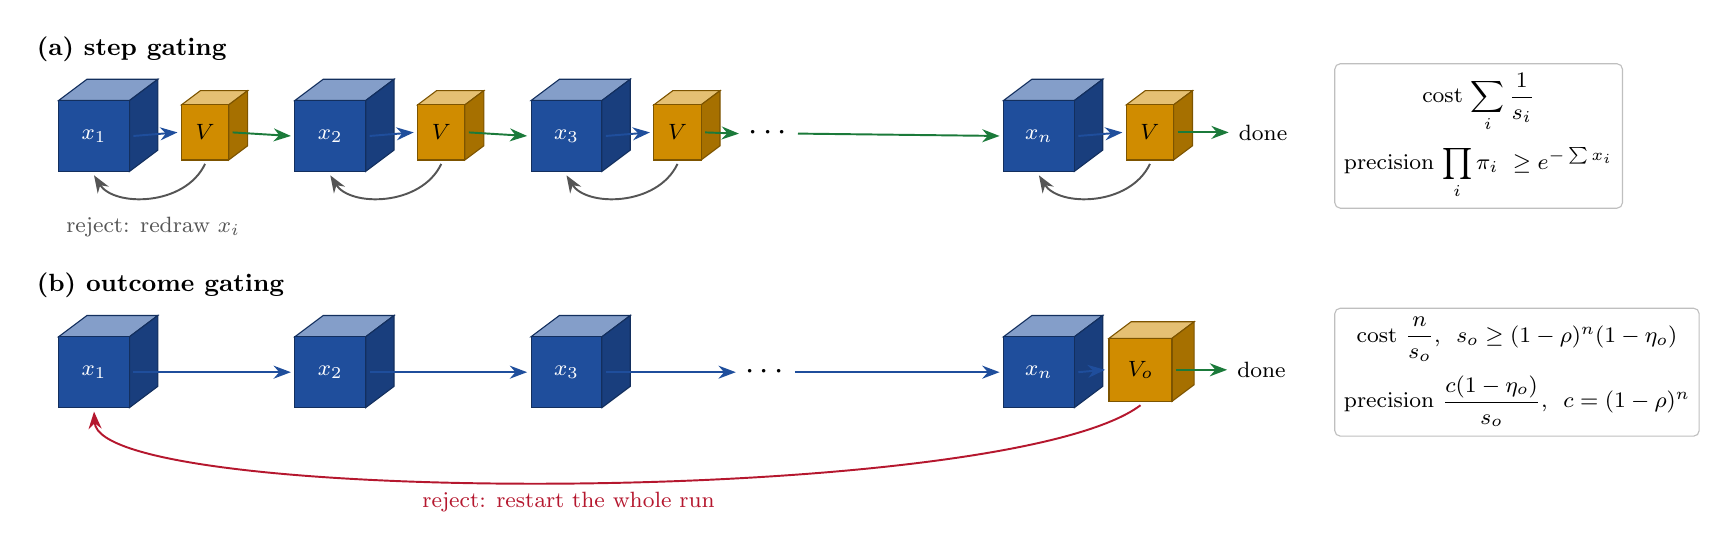
\begin{tikzpicture}[x={(1cm,0cm)},y={(0.4cm,0.3cm)},z={(0cm,1cm)},
  arr/.style={-{Stealth[length=2.2mm]},line width=0.7pt},
  lab/.style={font=\footnotesize,align=center}]
% ---------- step gating (top row)
\node[font=\small\bfseries,anchor=west] at (-0.4,0,4.55) {(a) step gating};
\foreach \i/\lab in {0/1,1/2,2/3,4/n}{
  \pgfmathsetmacro\xx{3.0*\i}
  \cuboid{\xx}{0}{3.0}{0.9}{0.9}{0.9}{cblue}
  \node[lab,white] at (\xx+0.45,0,3.45) {$x_{\lab}$};
  \cuboid{\xx+1.5}{0.15}{3.1}{0.6}{0.6}{0.7}{cgold}
  \node[lab] at (\xx+1.8,0.15,3.45) {$V$};
  \draw[arr,cblue] (\xx+0.95,0,3.45) -- (\xx+1.45,0.15,3.45);
  \draw[arr,cgrey] (\xx+1.8,0.15,3.05) .. controls (\xx+1.6,0,2.55) and (\xx+0.7,0,2.55) .. (\xx+0.45,0,2.95);
}
\foreach \i in {0,1}{\pgfmathsetmacro\xx{3.0*\i}\draw[arr,cgreen] (\xx+2.15,0.15,3.45) -- (\xx+2.95,0,3.45);}
\draw[arr,cgreen] (8.15,0.15,3.45) -- (8.6,0.1,3.45);
\node[font=\large] at (9.0,0.1,3.45) {$\cdots$};
\draw[arr,cgreen] (9.35,0.1,3.45) -- (11.95,0,3.45);
\draw[arr,cgreen] (14.15,0.15,3.45) -- (14.8,0.15,3.45) node[right,lab,black] {done};
\node[lab,cgrey] at (1.2,0,2.3) {reject: redraw $x_i$};
\node[lab,anchor=west,draw=gray!50,fill=white,rounded corners=2pt] at (16.2,0,3.45)
 {cost $\displaystyle\sum_{i}\frac{1}{s_i}$\\[4pt] precision $\displaystyle\prod_i\pi_i\ \ge e^{-\sum x_i}$};
% ---------- outcome gating (bottom row)
\node[font=\small\bfseries,anchor=west] at (-0.4,0,1.55) {(b) outcome gating};
\foreach \i/\lab in {0/1,1/2,2/3,4/n}{
  \pgfmathsetmacro\xx{3.0*\i}
  \cuboid{\xx}{0}{0}{0.9}{0.9}{0.9}{cblue}
  \node[lab,white] at (\xx+0.45,0,0.45) {$x_{\lab}$};}
\foreach \i in {0,1}{\pgfmathsetmacro\xx{3.0*\i}\draw[arr,cblue] (\xx+0.95,0,0.45) -- (\xx+2.95,0,0.45);}
\draw[arr,cblue] (6.95,0,0.45) -- (8.6,0,0.45);
\node[font=\large] at (9.0,0,0.45) {$\cdots$};
\draw[arr,cblue] (9.35,0,0.45) -- (11.95,0,0.45);
\cuboid{13.3}{0.1}{0.05}{0.8}{0.7}{0.8}{cgold}
\node[lab] at (13.7,0.1,0.45) {$V_o$};
\draw[arr,cblue] (12.95,0,0.45) -- (13.25,0.1,0.45);
\draw[arr,cgreen] (14.15,0.1,0.45) -- (14.8,0.1,0.45) node[right,lab,black] {done};
\draw[arr,cred] (13.7,0.1,0.0) .. controls (12.5,-1.2,-0.9) and (1.0,-1.2,-0.9) .. node[below,lab,cred] {reject: restart the whole run} (0.45,0,-0.05);
\node[lab,anchor=west,draw=gray!50,fill=white,rounded corners=2pt] at (16.2,0,0.45)
 {cost $\displaystyle\frac{n}{s_o}$, \ $s_o\ge(1-\rho)^n(1-\eta_o)$\\[4pt] precision $\displaystyle\frac{c(1-\eta_o)}{s_o}$, \ $c=(1-\rho)^n$};
\end{tikzpicture}
\end{document}
